\documentclass{ximera}

%\usepackage{todonotes}

\newcommand{\todo}{}

\usepackage{esint} % for \oiint
\ifxake%%https://math.meta.stackexchange.com/questions/9973/how-do-you-render-a-closed-surface-double-integral
\renewcommand{\oiint}{{\large\bigcirc}\kern-1.56em\iint}
\fi


\graphicspath{
  {./}
  {ximeraTutorial/}
  {basicPhilosophy/}
  {functionsOfSeveralVariables/}
  {normalVectors/}
  {lagrangeMultipliers/}
  {vectorFields/}
  {greensTheorem/}
  {shapeOfThingsToCome/}
  {dotProducts/}
  {partialDerivativesAndTheGradientVector/}
  {../productAndQuotientRules/exercises/}
  {../normalVectors/exercisesParametricPlots/}
  {../continuityOfFunctionsOfSeveralVariables/exercises/}
  {../partialDerivativesAndTheGradientVector/exercises/}
  {../directionalDerivativeAndChainRule/exercises/}
  {../commonCoordinates/exercisesCylindricalCoordinates/}
  {../commonCoordinates/exercisesSphericalCoordinates/}
  {../greensTheorem/exercisesCurlAndLineIntegrals/}
  {../greensTheorem/exercisesDivergenceAndLineIntegrals/}
  {../shapeOfThingsToCome/exercisesDivergenceTheorem/}
  {../greensTheorem/}
  {../shapeOfThingsToCome/}
  {../separableDifferentialEquations/exercises/}
  {vectorFields/}
}

\newcommand{\mooculus}{\textsf{\textbf{MOOC}\textnormal{\textsf{ULUS}}}}

\usepackage{tkz-euclide}
\usepackage{tikz}
\usepackage{tikz-cd}
\usetikzlibrary{arrows}
\tikzset{>=stealth,commutative diagrams/.cd,
  arrow style=tikz,diagrams={>=stealth}} %% cool arrow head
\tikzset{shorten <>/.style={ shorten >=#1, shorten <=#1 } } %% allows shorter vectors

\usetikzlibrary{backgrounds} %% for boxes around graphs
\usetikzlibrary{shapes,positioning}  %% Clouds and stars
\usetikzlibrary{matrix} %% for matrix
\usepgfplotslibrary{polar} %% for polar plots
\usepgfplotslibrary{fillbetween} %% to shade area between curves in TikZ
%\usetkzobj{all}
\usepackage[makeroom]{cancel} %% for strike outs
%\usepackage{mathtools} %% for pretty underbrace % Breaks Ximera
%\usepackage{multicol}
\usepackage{pgffor} %% required for integral for loops



%% http://tex.stackexchange.com/questions/66490/drawing-a-tikz-arc-specifying-the-center
%% Draws beach ball
\tikzset{pics/carc/.style args={#1:#2:#3}{code={\draw[pic actions] (#1:#3) arc(#1:#2:#3);}}}



\usepackage{array}
\setlength{\extrarowheight}{+.1cm}
\newdimen\digitwidth
\settowidth\digitwidth{9}
\def\divrule#1#2{
\noalign{\moveright#1\digitwidth
\vbox{\hrule width#2\digitwidth}}}




% \newcommand{\RR}{\mathbb R}
% \newcommand{\R}{\mathbb R}
% \newcommand{\N}{\mathbb N}
% \newcommand{\Z}{\mathbb Z}

\newcommand{\sagemath}{\textsf{SageMath}}


%\renewcommand{\d}{\,d\!}
%\renewcommand{\d}{\mathop{}\!d}
%\newcommand{\dd}[2][]{\frac{\d #1}{\d #2}}
%\newcommand{\pp}[2][]{\frac{\partial #1}{\partial #2}}
% \renewcommand{\l}{\ell}
%\newcommand{\ddx}{\frac{d}{\d x}}

% \newcommand{\zeroOverZero}{\ensuremath{\boldsymbol{\tfrac{0}{0}}}}
%\newcommand{\inftyOverInfty}{\ensuremath{\boldsymbol{\tfrac{\infty}{\infty}}}}
%\newcommand{\zeroOverInfty}{\ensuremath{\boldsymbol{\tfrac{0}{\infty}}}}
%\newcommand{\zeroTimesInfty}{\ensuremath{\small\boldsymbol{0\cdot \infty}}}
%\newcommand{\inftyMinusInfty}{\ensuremath{\small\boldsymbol{\infty - \infty}}}
%\newcommand{\oneToInfty}{\ensuremath{\boldsymbol{1^\infty}}}
%\newcommand{\zeroToZero}{\ensuremath{\boldsymbol{0^0}}}
%\newcommand{\inftyToZero}{\ensuremath{\boldsymbol{\infty^0}}}



% \newcommand{\numOverZero}{\ensuremath{\boldsymbol{\tfrac{\#}{0}}}}
% \newcommand{\dfn}{\textbf}
% \newcommand{\unit}{\,\mathrm}
% \newcommand{\unit}{\mathop{}\!\mathrm}
% \newcommand{\eval}[1]{\bigg[ #1 \bigg]}
% \newcommand{\seq}[1]{\left( #1 \right)}
% \renewcommand{\epsilon}{\varepsilon}
% \renewcommand{\phi}{\varphi}


% \renewcommand{\iff}{\Leftrightarrow}

% \DeclareMathOperator{\arccot}{arccot}
% \DeclareMathOperator{\arcsec}{arcsec}
% \DeclareMathOperator{\arccsc}{arccsc}
% \DeclareMathOperator{\si}{Si}
% \DeclareMathOperator{\scal}{scal}
% \DeclareMathOperator{\sign}{sign}


%% \newcommand{\tightoverset}[2]{% for arrow vec
%%   \mathop{#2}\limits^{\vbox to -.5ex{\kern-0.75ex\hbox{$#1$}\vss}}}
% \newcommand{\arrowvec}[1]{{\overset{\rightharpoonup}{#1}}}
% \renewcommand{\vec}[1]{\arrowvec{\mathbf{#1}}}
% \renewcommand{\vec}[1]{{\overset{\boldsymbol{\rightharpoonup}}{\mathbf{#1}}}}

% \newcommand{\point}[1]{\left(#1\right)} %this allows \vector{ to be changed to \vector{ with a quick find and replace
% \newcommand{\pt}[1]{\mathbf{#1}} %this allows \vec{ to be changed to \vec{ with a quick find and replace
% \newcommand{\Lim}[2]{\lim_{\point{#1} \to \point{#2}}} %Bart, I changed this to point since I want to use it.  It runs through both of the exercise and exerciseE files in limits section, which is why it was in each document to start with.

% \DeclareMathOperator{\proj}{\mathbf{proj}}
% \newcommand{\veci}{{\boldsymbol{\hat{\imath}}}}
% \newcommand{\vecj}{{\boldsymbol{\hat{\jmath}}}}
% \newcommand{\veck}{{\boldsymbol{\hat{k}}}}
% \newcommand{\vecl}{\vec{\boldsymbol{\l}}}
% \newcommand{\uvec}[1]{\mathbf{\hat{#1}}}
% \newcommand{\utan}{\mathbf{\hat{t}}}
% \newcommand{\unormal}{\mathbf{\hat{n}}}
% \newcommand{\ubinormal}{\mathbf{\hat{b}}}

% \newcommand{\dotp}{\bullet}
% \newcommand{\cross}{\boldsymbol\times}
% \newcommand{\grad}{\boldsymbol\nabla}
% \newcommand{\divergence}{\grad\dotp}
% \newcommand{\curl}{\grad\cross}
%\DeclareMathOperator{\divergence}{divergence}
%\DeclareMathOperator{\curl}[1]{\grad\cross #1}
% \newcommand{\lto}{\mathop{\longrightarrow\,}\limits}

% \renewcommand{\bar}{\overline}

\colorlet{textColor}{black}
\colorlet{background}{white}
\colorlet{penColor}{blue!50!black} % Color of a curve in a plot
\colorlet{penColor2}{red!50!black}% Color of a curve in a plot
\colorlet{penColor3}{red!50!blue} % Color of a curve in a plot
\colorlet{penColor4}{green!50!black} % Color of a curve in a plot
\colorlet{penColor5}{orange!80!black} % Color of a curve in a plot
\colorlet{penColor6}{yellow!70!black} % Color of a curve in a plot
\colorlet{fill1}{penColor!20} % Color of fill in a plot
\colorlet{fill2}{penColor2!20} % Color of fill in a plot
\colorlet{fillp}{fill1} % Color of positive area
\colorlet{filln}{penColor2!20} % Color of negative area
\colorlet{fill3}{penColor3!20} % Fill
\colorlet{fill4}{penColor4!20} % Fill
\colorlet{fill5}{penColor5!20} % Fill
\colorlet{gridColor}{gray!50} % Color of grid in a plot

\newcommand{\surfaceColor}{violet}
\newcommand{\surfaceColorTwo}{redyellow}
\newcommand{\sliceColor}{greenyellow}




\pgfmathdeclarefunction{gauss}{2}{% gives gaussian
  \pgfmathparse{1/(#2*sqrt(2*pi))*exp(-((x-#1)^2)/(2*#2^2))}%
}


%%%%%%%%%%%%%
%% Vectors
%%%%%%%%%%%%%

%% Simple horiz vectors
\renewcommand{\vector}[1]{\left\langle #1\right\rangle}


%% %% Complex Horiz Vectors with angle brackets
%% \makeatletter
%% \renewcommand{\vector}[2][ , ]{\left\langle%
%%   \def\nextitem{\def\nextitem{#1}}%
%%   \@for \el:=#2\do{\nextitem\el}\right\rangle%
%% }
%% \makeatother

%% %% Vertical Vectors
%% \def\vector#1{\begin{bmatrix}\vecListA#1,,\end{bmatrix}}
%% \def\vecListA#1,{\if,#1,\else #1\cr \expandafter \vecListA \fi}

%%%%%%%%%%%%%
%% End of vectors
%%%%%%%%%%%%%

%\newcommand{\fullwidth}{}
%\newcommand{\normalwidth}{}



%% makes a snazzy t-chart for evaluating functions
%\newenvironment{tchart}{\rowcolors{2}{}{background!90!textColor}\array}{\endarray}

%%This is to help with formatting on future title pages.
\newenvironment{sectionOutcomes}{}{}



%% Flowchart stuff
%\tikzstyle{startstop} = [rectangle, rounded corners, minimum width=3cm, minimum height=1cm,text centered, draw=black]
%\tikzstyle{question} = [rectangle, minimum width=3cm, minimum height=1cm, text centered, draw=black]
%\tikzstyle{decision} = [trapezium, trapezium left angle=70, trapezium right angle=110, minimum width=3cm, minimum height=1cm, text centered, draw=black]
%\tikzstyle{question} = [rectangle, rounded corners, minimum width=3cm, minimum height=1cm,text centered, draw=black]
%\tikzstyle{process} = [rectangle, minimum width=3cm, minimum height=1cm, text centered, draw=black]
%\tikzstyle{decision} = [trapezium, trapezium left angle=70, trapezium right angle=110, minimum width=3cm, minimum height=1cm, text centered, draw=black]


\title{Polynomial Analysis}

\begin{document}

\begin{abstract}
the polynomial story
\end{abstract}
\maketitle







Let's run through the analysis plan for polynomials.





$\blacktriangleright$ \textbf{\textcolor{red!10!blue!90!}{Domain:}} \\ 
The natural domain of a polynomial function is all real numbers.  Of course, a particular polynomial function may be defined with a restricted domain.



It just turns out that the standard form for a polynomial is just not that helpful.  Our analysis prefers a factored form. \\




\begin{formula} \textbf{\textcolor{purple!85!blue}{Forms}}

Formulas for polynomial functions have two forms:



\begin{itemize}
\item \textbf{\textcolor{purple!85!blue}{Standard Form:}}   The standard form for a polynomial function is a \textbf{\textcolor{purple!85!blue}{sum}}. It looks like 
\[ a_n x^n + a_{n-1} x^{n-1} + \cdots + a_2 x^2 + a_1 x + a_0 \]
\item \textbf{\textcolor{purple!85!blue}{Factored Form:}}  The factored form for a polynomial function is a \textbf{\textcolor{purple!85!blue}{product}}. It looks like 
\[ a(x - r_n)(x - r_{n-1}) \cdots (x - r_1) \]
\end{itemize}


\end{formula}
We prefer the factored form for our function analysis.    The standard form is just not that helpful for function analysis. \\

\textbf{Note:} A polynomial may have repeated zeros.  For this reason, the factored form usually collects like factors:


\[   a (x - r_k)^{e_k} (x - r_{k-1})^{e_{k-1}} \cdots (x - r_1)^{e_1}             \]


Here, the zeros are distinct:  $r_i \ne r_j$ when $i \ne j$.

The exponents are called \textbf{\textcolor{purple!85!blue}{multiplicities}} of the zeros or the factors. 






$\blacktriangleright$   \textbf{\textcolor{red!10!blue!90!}{Roots and Zeros:}} \\ 
\textbf{Zeros} of polynomials are also called \textbf{roots} of the polynomials.  A polynomial function behaves in one of two ways around a root.

\begin{itemize}
\item If the multiplicity is odd then the function changes sign over the root.  The graph crosses over the horizontal axis at the corresponding intercept.
\item If the multiplicity is even then the function does not change sign over the root.  The graph does not cross over the horizontal axis at the corresponding intercept. Instead, it bounces back in the direction from which it came.
\end{itemize}


\textbf{Constant functions} are polynomial functions.  They don't have zeros, unless the constant function just happens to be the zero constant function.  \\


\textbf{Linear functions} are polynomial functions. They have one real root, unless it is a constant function.  You can solve for this root. \\


\textbf{Quadratic functions} are polynomial functions. They have $0$, $1$, or $2$ real roots.  You can solve for these real roots. \\


\textbf{Higher Order Polynomials} are polynomial functions with degree $3$ or greater.  We do not have quick formulas to obtain their roots.  Our usual strategy is to factor, if we can.  





$\blacktriangleright$ \textbf{\textcolor{red!10!blue!90!}{Continuity:}} \\ 
Polynomials are nice functions.  They are continuous everywhere.  They have no discontinuities or singularities.







$\blacktriangleright$ \textbf{\textcolor{red!10!blue!90!}{Behavior(Rate-of-Change):}} \\ 
The critical numbers partition the real line into intervals where the polynomial function increases or decreases.  All of this depends on getting the critical numbers, which will require a derivative.










$\blacktriangleright$  \textbf{\textcolor{red!10!blue!90!}{Extrema (Maximums and Minimums):}} \\ 
Polynomial functions can have global and local maximums and/or minimums, which our algebra is unlikely to identify. \\

 In Calculus, when we have a derivative, then we can attempt to locate exact values of \textbf{critical numbers}.  Without the derivative, we turn to technology for some assistance in approximating.  That's the best we can do.






$\blacktriangleright$  \textbf{\textcolor{red!10!blue!90!}{Range:}} \\ 

Unless the polynomial is a constant function, polynomials are unbounded.  The range will include $-\infty$ or $\infty$ or both.  

The range of a polynomial with an odd degree is $(-\infty, \infty)$. \\


The range of a polynomial with an even degree is of the form $(-\infty, m]$ or $[m, \infty)$, for some real number $m$.  Generally speaking, figuring out the exact value of $m$ for any particular polynomial will need Calculus\\










\begin{center}

A random polynomial is almost impossible to accurately analyze. Our algebra is not strong enough.


Unless the polynomial is special (can be factored nicely), then approximating with a graph is usually unavoidable.

\end{center}



$\blacktriangleright$ \textbf{\textcolor{red!10!blue!90!}{Graphs:}} \\ 
Graphs of polynomials are nice.  They are smooth.  They do not have corners or spikes or breaks or asymptotes. Once we have the roots, we can plot the intercepts.  Then we can smoothly connect them according to their multiplicities and have a pretty good sketch of the shape of the graph.

With a basic general shape, we can estimate critical numbers and types of extrema values.




















\begin{example} Polynomial


Completely analyze $p(w) = -\frac{1}{5}(w+4)(w-3)(w-3)$


First, let's collect like factors: $p(w) = -\frac{1}{5}(w+4)(w-3)^2$.


This formula matches our template for a polynomial in factored form. \\

\textbf{Domain}

Since, $p$ is a polynomial function, its natural domain is $(-\infty, \infty)$. \\



\textbf{Zeros}



$p$ is a polynomial of degree $3$ and we can see from its factorization that it has two roots, $-4$ and $3$. \\  




\textbf{Continuity}

Since, $p$ is a polynomial function, it is continuous. \\



\textbf{End-Behavior}


The end-behavior of $p$ is dictated by the leading term and the degree, $-\frac{1}{5} w^3$.  

An odd degree tells us that the two directions will have different signs for the end-behavior.  The negative leading coefficient tells us that the polynomial is unbounded negatively in the positive direction.


\[
\lim\limits_{w \to \infty}p(w) = -\infty
\]


\[
\lim\limits_{w \to -\infty}p(w) = \infty
\] 






\textbf{Behavior}

We can't get the behavior exactly.  We need the derivative for that. We can get an approximate idea.

Since $p(w)$ is a polynomial, these roots (zeros) are the only candidates for where $p(w)$ might change signs.  The multiplicity will tell us if $p(w)$ changes sign at each root. If we can determine the sign of $p(w)$ anywhere, then we'll know the sign of $p(w)$ everywhere.\\

\begin{itemize}
\item $-4$ is a root of multiplicity $\answer{1}$.  Since this multiplicity is odd, $p$ will \wordChoice{\choice[correct]{change sign} \choice{not change sign}} through $-4$ and the graph will cross at $(-4,0)$.
\item $3$ is a root of multiplicity $\answer{2}$.  Since this multiplicity is even, $p$ will \wordChoice{\choice{change sign} \choice[correct]{not change sign}} through $3$ and the graph will not cross at $(3,0)$.  The graph will touch and then bounce back.
\end{itemize}





Let's collect our ideas graphically.


\begin{image}
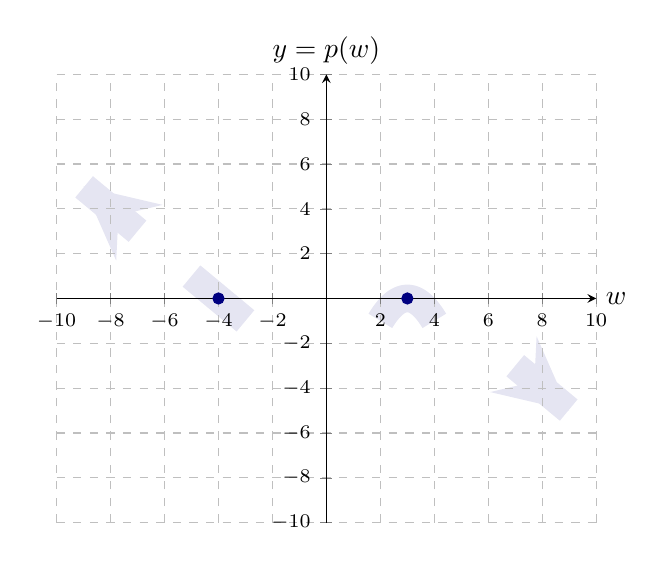
\begin{tikzpicture}
  \begin{axis}[
            domain=-10:10, ymax=10, xmax=10, ymin=-10, xmin=-10,
            axis lines =center, xlabel=$w$, ylabel={$y=p(w)$}, grid = major, grid style={dashed},
            ytick={-10,-8,-6,-4,-2,2,4,6,8,10},
            xtick={-10,-8,-6,-4,-2,2,4,6,8,10},
            yticklabels={$-10$,$-8$,$-6$,$-4$,$-2$,$2$,$4$,$6$,$8$,$10$}, 
            xticklabels={$-10$,$-8$,$-6$,$-4$,$-2$,$2$,$4$,$6$,$8$,$10$},
            ticklabel style={font=\scriptsize},
            every axis y label/.style={at=(current axis.above origin),anchor=south},
            every axis x label/.style={at=(current axis.right of origin),anchor=west},
            axis on top
          ]
          
          %\addplot [line width=2, penColor2, smooth,samples=100,domain=(-6:2)] {-2*x-3};


          %\addplot [<-, line width=10, penColor!10!background] plot coordinates {(-2,-25) (-1,7)}; 



            \addplot [line width=10, penColor!10!background, smooth,samples=100,domain=(-9:-7),<-] {-(x+4)};
            \addplot [line width=10, penColor!10!background, smooth,samples=100,domain=(-5:-3)] {-(x+4)};
            \addplot [line width=10, penColor!10!background, smooth,samples=100,domain=(2:4)] {-(x-3)^2)};
            \addplot [line width=10, penColor!10!background, smooth,samples=100,domain=(7:9),->] {-(x-4)};

          %\addplot[color=penColor,fill=penColor2,only marks,mark=*] coordinates{(-6,9)};
          %\addplot[color=penColor,fill=penColor2,only marks,mark=*] coordinates{(2,-7)};

          \addplot[color=penColor,fill=penColor,only marks,mark=*] coordinates{(-4,0)};
          \addplot[color=penColor,fill=penColor,only marks,mark=*] coordinates{(3,0)};


           

  \end{axis}
\end{tikzpicture}
\end{image}




The graph is very suggestive that there is a local minimum somewhere around $-1$ and a local maximum at $3$.  \\


$3$ is a zero, $p(3) = 0$. In addition, $p$ is negative around $3$.  That makes $p(3) = 0$ a local maximum.  That makes $3$ a critical number as well.






\begin{image}
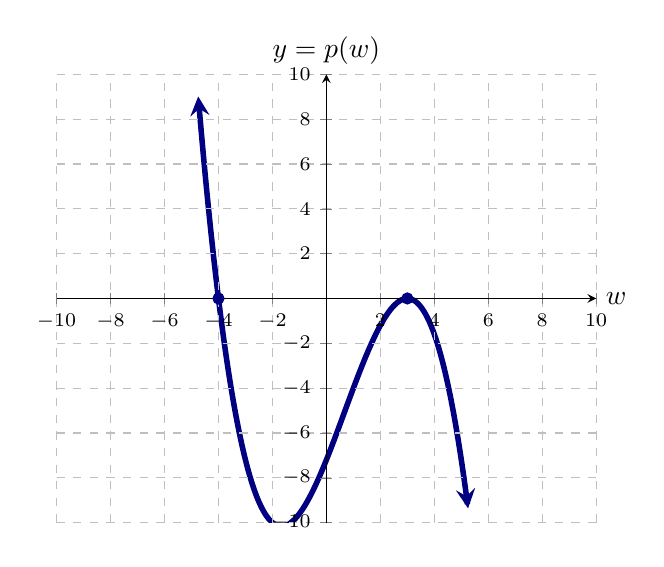
\begin{tikzpicture}
  \begin{axis}[
            domain=-10:10, ymax=10, xmax=10, ymin=-10, xmin=-10,
            axis lines =center, xlabel=$w$, ylabel={$y=p(w)$}, grid = major, grid style={dashed},
            ytick={-10,-8,-6,-4,-2,2,4,6,8,10},
            xtick={-10,-8,-6,-4,-2,2,4,6,8,10},
            yticklabels={$-10$,$-8$,$-6$,$-4$,$-2$,$2$,$4$,$6$,$8$,$10$}, 
            xticklabels={$-10$,$-8$,$-6$,$-4$,$-2$,$2$,$4$,$6$,$8$,$10$},
            ticklabel style={font=\scriptsize},
            every axis y label/.style={at=(current axis.above origin),anchor=south},
            every axis x label/.style={at=(current axis.right of origin),anchor=west},
            axis on top
          ]
          
          %\addplot [line width=2, penColor2, smooth,samples=100,domain=(-6:2)] {-2*x-3};
            \addplot [line width=2, penColor, smooth,samples=300,domain=(-4.75:5.25),<->] {-0.2*(x+4)*(x-3)^2};


          %\addplot[color=penColor,fill=penColor2,only marks,mark=*] coordinates{(-6,9)};
          %\addplot[color=penColor,fill=penColor2,only marks,mark=*] coordinates{(2,-7)};

          \addplot[color=penColor,fill=penColor,only marks,mark=*] coordinates{(-4,0)};
          \addplot[color=penColor,fill=penColor,only marks,mark=*] coordinates{(3,0)};


           

  \end{axis}
\end{tikzpicture}
\end{image}

With some technology, we can approximate the other critical number to be $-1.67$ and the local minimum to be $-10.163$.


\begin{itemize}
\item $p$ is \wordChoice{\choice{increasing} \choice[correct]{decreasing}}  on $(-\infty, -1.67]$.
\item $p$ is \wordChoice{\choice[correct]{increasing} \choice{decreasing}}  on $[-1.67, 3]$.
\item $p$ is \wordChoice{\choice{increasing} \choice[correct]{decreasing}}  on $[3, \infty)$.
\end{itemize}



There is no global maximum or minimum, because  $\lim\limits_{w \to -\infty}p(w) = \infty$ and $\lim\limits_{w \to \infty}p(w) = -\infty$. 


That's as close as we are going to get it. \\

\end{example}

















\subsection*{with the Derivative}


Once we have a function's derivative, we can get the exact values of the critical numbers. \\


Calculus will tell us how to get the derivative of any function.  In Precalculus, you can get the derivative of a linear function or a quadratic funciton.  You cannot get the derivative of any other polynomial.\\

But, you could be given the derivative and use it to find exat values of critical numbers. \\




Calculus would give us the derivative, $p'(w) = -\frac{1}{5}(3w^2 - 4w - 15)$. \\

$p'(x)$ is another polynomial. The zeros of this derivative would be critical numbers of $p(x)$.  $p'(w)$ is a quadratic.  Therefore, we can obtain its zeros, the critical numbers of $p(x)$, via the quadratic formula.


\[  \frac{4 \pm \sqrt{(-4)^2 - 4 \cdot 3 \cdot (-15)}}{2 \cdot 3} =    \frac{4 \pm \sqrt{196}}{6}  = \frac{4 \pm 14}{6}       \]

We get two real roots: $\frac{4 + 14}{6} = \frac{18}{6} = 3$  and $\frac{4 - 14}{6} = \frac{-10}{6} = \frac{-5}{3} \approx -1.67$




This allows us to factor the derivative

\[
p'(w) = -\frac{3}{5}(w - 3) \left( w + \frac{5}{3} \right)
\]

Each of these roots or factors has a multiplicy of $1$, which means $p'(w)$ changes signs over $-\frac{5}{3}$ and $3$. \\


$p'(w)$ is a polynomial, which means it is continuous. It is certainly negative for very large negative values of $w$.  Then it changes sign over $-\frac{5}{3}$.  So, $p'(w)$ is positive between $-\frac{5}{3}$ and $3$.  Then, it changes sign to negative at $3$.





\begin{itemize}
\item $p$ decreases on $\left(-\infty, \frac{-5}{3}\right]$.
\item $p$ increases on $\left[\frac{-5}{3}, 3\right]$.
\item $p$ decreases on $[3, \infty)$.
\end{itemize}



Another approach to obtaining the roots of $p'(w) = \frac{1}{5}(3w^2 - 4w - 15)$ would be to factor. 


\[
3w^2 - 4w - 15      = (A \cdot w + B)(C \cdot w + D) 
\]

$A \cdot C = 3$ and $3$ is a prime number.  Therefore, one of $A$ and $C$ is $3$ and the other is $1$.



\[
3w^2 - 4w - 15      = (w + B)(3 \, w + D) 
\]



$B \cdot D = -15$.  A first guess is that one of $B$ and $D$ is $-5$ and the other is $3$. 


\[
3w^2 - 4w - 15      = (w - 5)(3 \, w + 3) = 3 \, w^2 -12 \, w - 15
\]



Let's try it the other way, $-3$ and the other is $5$.



\[
3w^2 - 4w - 15     = (w - 3)(3 \, w + 5) = 3 \, w^2  -4 \, w - 15
\]



That worked. \\



$p'(w) = \frac{1}{5}(3w^2 - 4w - 15) = \frac{1}{5} (w - 3)(3 \, w + 5)$. \\


That tells us that $3$ and $-\frac{5}{3}$ are the critical numbers of $p(x)$.






\begin{center}
\textbf{\textcolor{green!50!black}{ooooo-=-=-=-ooOoo-=-=-=-ooooo}} \\

more examples can be found by following this link\\ \link[More Examples of Poynomial and Rational functions]{https://ximera.osu.edu/csccmathematics/precalculus/precalculus/polynomialFunctions/examples/exampleList}

\end{center}






\end{document}
